\chapter{动态博弈}\label{chap:dynamical-game}

本章我们讨论每个玩家需要操作多次的博弈,此时,博弈被称为\textbf{动态博弈}\index{博弈!动态~}.

\section{输赢博弈}

\textbf{输赢博弈}\index{博弈!输赢~}指的是玩家的收益只能取两个值(输或赢)的博弈. 赢博弈中,每个游戏状态只有一个玩家可以进行操作的情况研究最多. 这种情况通常称为\textbf{扩展式博弈}\index{博弈!扩展式~}. 围棋、象棋、斗地主都是输赢博弈. 输赢博弈的分类见\Cref{tab:win-lose-game}.

\begin{table}[ht]
    \centering
    \begin{tabular}{cc}
        二人 & 多人 \\
        输赢 & 输赢平\\
        有限深 & 无穷深 \\
        完全信息 & 不完全信息 \\
        非合作 & 合作
    \end{tabular}
    \caption{输赢博弈的分类.}
    \label{tab:win-lose-game}
\end{table}

\begin{example}
    斗地主是一个多人有限轮不完全信息合作输赢博弈.
\begin{figure}
    \centering
    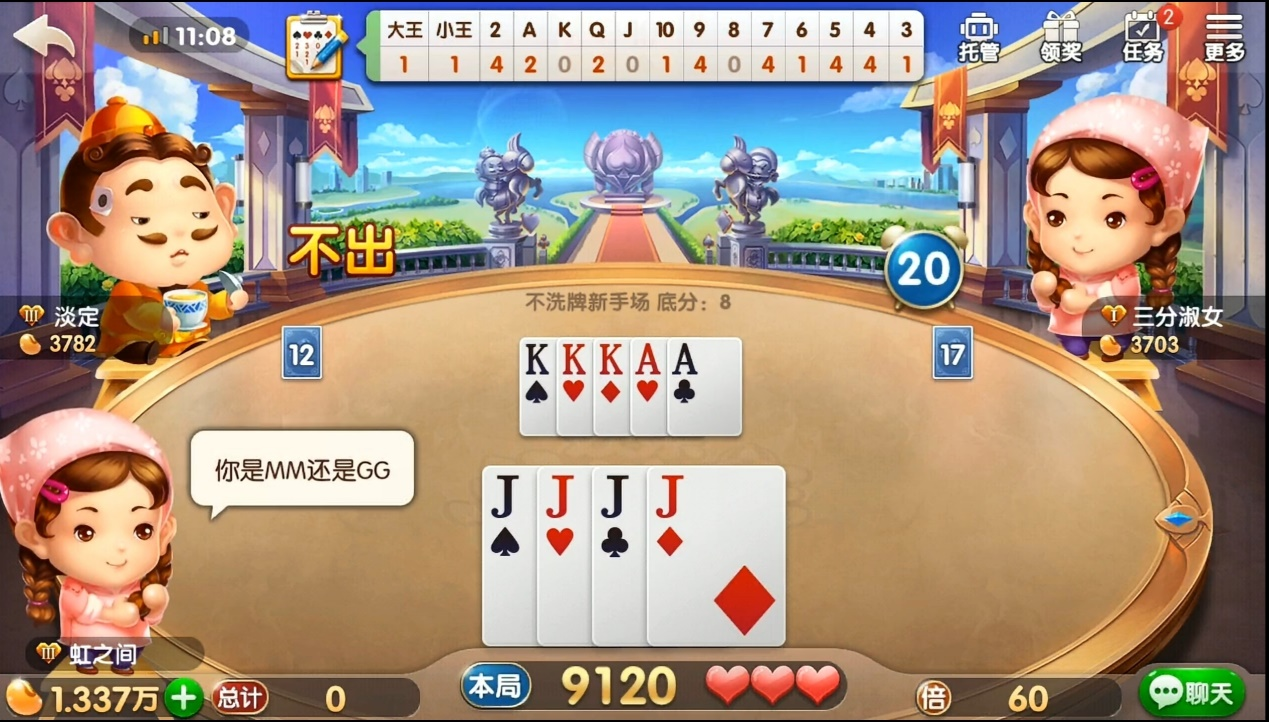
\includegraphics[width=0.75\textwidth]{Chapters/dynamical-game/figures/fight-landlord.jpg}
    \caption{斗地主.}
\end{figure}

\end{example}

我们在本部分主要关注最简单的一种博弈,即\emph{完全信息确定性回合制博弈}\index{博弈!完全信息确定性回合制~},与之相关的概念如下:
\begin{itemize}
    \item \emph{局面}\index{局面}:博弈的状态包括博弈本身的状态(棋盘状态、出牌情况等)和当前回合是哪个玩家.
    \item (无记忆)\emph{策略}\index{策略}:从局面到行动空间的映射$s_i:C\to\mathcal A$.
    \item \emph{确定性}\index{确定性}:给定当前格局和所有玩家的行动,可以唯一确定下一回合的格局.
    \item  \emph{完全信息}\index{完全信息}:所有玩家都知道当前局面,都知道每个玩家的行动,并且这些是共同知识.
\end{itemize}

这样的博弈可以用博弈树表示出来,例如,井字棋的博弈树见\Cref{fig:gametree}.

\begin{figure}
    \centering
    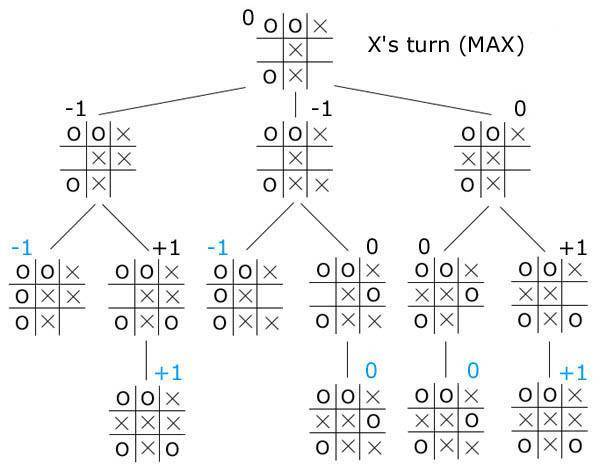
\includegraphics[scale=0.4]{Chapters/dynamical-game/figures/gametree.jpg}
    \caption{井字棋的博弈树.}
    \label{fig:gametree}
\end{figure}

输赢博弈一个自然的问题是:玩家是否总可以获胜?这就涉及到\emph{必胜策略}\index{必胜策略}的概念:无论对手如何进行行动,玩家都可以取得胜利的策略. 必胜策略是一种\emph{解概念}\index{解概念},即给定一个博弈,求解具有一定性质的玩家策略. 如果某个玩家具有必胜策略,那么我们就说这个博弈是\emph{被决定的}\index{博弈!被决定的~}. 什么博弈是被决定的?这一问题的答案由Zermelo定理给出.

\begin{theorem}[Zermelo定理, Von Neumann]\label{thm:zermelo}\index{Zermelo定理}
如果一个博弈是双人的、有限深的、确定的、完全信息的、输赢的,那么这个博弈是被决定的.
\end{theorem}
以上限定词缺一不可,缺少了任何一个都可能导致结论不成立.

\begin{proof}[证明一:逻辑证明]
设$W_i$表示“玩家$i$获胜”, $i=1,2$. 于是$x\in W_1\iff x\not\in W_2$.

先手玩家有必胜策略当且仅当
\[\exists a_0\forall b_0\exists a_1\forall b_1\dots\exists a_n\forall b_n: (a_0b_0\dots a_nb_n)\in W_1.\]

后手玩家有必胜策略当且仅当
\[\forall a_0\exists b_0\forall a_1\exists b_1\dots\forall a_n\exists b_n: (a_0b_0\dots a_nb_n)\in W_2.\]

两个命题互为否定,因此二者恰有一个成立!
\end{proof}

\begin{proof}[证明二:后向归纳法]
从博弈树的叶节点往根节点推理.

如果此节点是玩家$i$的回合,那么往后一轮的局面已经完全确定.
\begin{itemize}
    \item 如果有一种走法使得玩家$i$必胜,那么玩家$i$选择这种走法即可.
    \item 否则,玩家$i$无论如何也不可能获胜.
\end{itemize}

当到达到根节点的时候,有一方有必胜策略,另一方必输.

这种证明方式被称为\emph{后向归纳法}\index{后向归纳法}:从最后一期开始往前推理,最终确定一个解概念.
\end{proof}

如果博弈的结局还有平局,我们有如下Zermelo定理:
\begin{theorem}[有平局的Zermelo定理]\label{thm:zermelo-draw}\index{Zermelo定理}
如果一个博弈是双人的、有限深的、确定的、完全信息的,博弈的结果有输赢平局三种,那么下面三条有且仅有一条成立:
\begin{itemize}
    \item 第一个玩家有必胜策略.
    \item 第二个玩家有必胜策略.
    \item 双方都有不败策略,因此完全理性的玩家在博弈中必然平局.
\end{itemize}
\end{theorem}
证明留做练习。

尽管Zermelo定理的第二个证明构造出了必胜策略,但是后向归纳法的搜索空间过于庞大. 例如,充分大但有限的棋盘上,五子棋先手玩家存在不败策略,但是没有经过训练的人类或者简单的算法先手不一定会胜利。究其原因,人的思考以及机器搜索的过程实际上是前向探索的过程. 如何进行搜索是取得胜利重要的因素. 其中一个非常震撼的例子就是AlphaGo的出现,机器战胜了人类围棋高手. 以下我们介绍AlphaGo的设计思路.

由Zermelo定理可知,围棋也存在必胜策略. 然而标准围棋棋盘大小为$19\times 19$,状态空间量级为$10^{170}$,过大的状态空间使得我们无法使用后向归纳法求解出必胜策略. DeepMind的AlphaGo\index{AlphaGo}、AlphaZero\index{AlphaZero}利用深度强化学习的方法取得了围棋博弈的出色表现. 以下我们探讨AlphaGo如何通过神经网络建模博弈的过程.

AlphaGo算法包含\emph{策略网络}\index{策略网络}, \emph{价值网络}\index{价值网络}和\emph{Monte-Carlo树搜索}\index{Monte-Carlo树搜索}\index{MCTS}(MCTS).
\begin{itemize}
    \item 策略网络和价值网络的输入为当前局面状态$s\in C$. 
    \item 策略网络的输出为下一步落子位置$a\in\mathcal A$(361维的one-hot向量).
    \item 价值网络的输出为该局面的价值评估(期望收益: 输$-1$/赢$+1$).
    \item MCTS利用策略网络进行\emph{扩展},使用价值网络进行\emph{评估},利用UCB公式返回最优的搜索结果作为落子决策.
\end{itemize}

AlphaGo使用模仿学习(人类专家对弈数据)、强化学习(自博弈,策略梯度)的方式训练策略网络,使用自我博弈过程中的数据监督训练价值网络.

\lhysays{仔细讨论这部分{关于输赢博弈的讨论}
\begin{itemize}
    \item 什么叫完全理性的玩家?
    \item 表示完整的策略需要多少比特?
    \item 是否有高效的算法计算必胜策略?
    \item 如果博弈多方不是完全对抗的(即零和),那么是否还有必胜策略?是否有其他合理的解概念?
\end{itemize}}

我们再看一个有趣的例子:\emph{对话博弈}\index{博弈!对话~}。在对话博弈中,我们可以把对命题$\phi$的辩论过程形式化为一个博弈. 博弈中有两个玩家,一个需要证明$\phi$是真的,被称为\emph{正方} $P$,一个需要说明$P$的论据是有矛盾的,它被称为\emph{反方} $O$. 两个玩家可以对命题的某个部分发起\emph{质疑},或者对某个质疑作出\emph{辩护}. 当正方成功辩护了所有的质疑,而反方已经无法再发出新的质疑,正方获胜;否则反方获胜.

我们以命题逻辑为例,考虑合取和蕴含. 感叹号$!$表示陈述,问号$?$表示询问. 当一个玩家$X$($P$或者$O$)说了一个合取式,另一个玩家$Y$如果想质疑,需要询问合取中的某个部分($L^\wedge$或$R^\wedge$). $X$需要陈述该部分对应的命题作为辩护. 这一规则可以总结为\Cref{tab:dialogue-game-or}.
\begin{table}[ht]
    \centering
    \begin{tabular}{c|c|c}
         陈述&质疑&辩护  \\\hline
         $X!\varphi\wedge\psi$&$Y?L^\wedge$或$Y?R^\wedge$& 对应地,$X!\varphi$或$X!\psi$
    \end{tabular}
    \caption{对话博弈的规则:合取}
    \label{tab:dialogue-game-or}
\end{table}

当一个玩家$X$($P$或者$O$)说了一个蕴含式,另一个玩家$Y$如果想质疑,需要陈述前提. $X$则需要陈述结论作为辩护. 这一规则可以总结为\Cref{tab:dialogue-game-impl}.
\begin{table}[ht]
    \centering
    \begin{tabular}{c|c|c}
         陈述&质疑&辩护  \\\hline
         $X!\varphi\to\psi$&$Y!\varphi$&$X!\psi$
    \end{tabular}
    \caption{对话博弈的规则:蕴含}
    \label{tab:dialogue-game-impl}
\end{table}

我们考虑一个具体的例子$(p\wedge q)\to p$. 用一个表格来表示辩论的过程,这个表格有两列,分别表示玩家$O$和$P$. 每个玩家分别有三列,$A$表示当前操作是第几步(两个玩家统一计数),$B$表示当前操作质疑的是哪一步,中间一列表示当前的操作(陈述或者询问).
\[
    \begin{array}{|c|c|c|c|c|c|}
    \hline
        \multicolumn{3}{|c|}{O} & \multicolumn{3}{|c|}{P} \\\hline
        A &  & B & B & & A\\\hline\hline
    \end{array}
\]

\newcommand{\gray}{\cellcolor{gray}}
玩家$P$陈述要辩论的命题.
\[
    \begin{array}{|c|c|c|c|c|c|}
    \hline
        \multicolumn{3}{|c|}{O} & \multicolumn{3}{|c|}{P} \\\hline
        &&&&\gray !p\wedge q\to p&\gray 0\\
        \hline
    \end{array}
\]
玩家$O$质疑这一陈述.
\[
    \begin{array}{|c|c|c|c|c|c|}
    \hline
        \multicolumn{3}{|c|}{O} & \multicolumn{3}{|c|}{P} \\\hline
        &&&&!p\wedge q\to p&0\\\hline
        \gray 1&\gray !p\wedge q&\gray (0)&&&\\\hline
    \end{array}
\]
现在又一次轮到了玩家$P$,他可以选择为蕴含式辩护,或者质疑这个合取式. 我们假设他这次选择质疑合取式,那么他需要询问左边或者右边,假设他询问了左边:
\[
    \begin{array}{|c|c|c|c|c|c|}
    \hline
        \multicolumn{3}{|c|}{O} & \multicolumn{3}{|c|}{P} \\\hline
        &&&&!p\wedge q\to p&0\\\hline
        1&!p\wedge q& (0)&&&\\\hline
        &&&\gray (1)&\gray ? L^\wedge &\gray 2\\\hline
    \end{array}
\]
现在轮到了玩家$O$. 他已经没有别的可以进行的操作了,只能对操作$2$进行辩护.
\[
    \begin{array}{|c|c|c|c|c|c|}
    \hline
        \multicolumn{3}{|c|}{O} & \multicolumn{3}{|c|}{P} \\\hline
        &&&&!p\wedge q\to p&0\\\hline
        1&!p\wedge q& (0)&&&\\\hline
        \gray 3&\gray !p&\gray &(1)&? L^\wedge &2\\\hline
    \end{array}
\]
现在轮到了玩家$P$. 他已经没有别的可以进行的操作了,只能对操作$1$进行辩护. 因为玩家$O$已经陈述了$p$,所以他可以用这个陈述来辩护.
\[
    \begin{array}{|c|c|c|c|c|c|}
    \hline
        \multicolumn{3}{|c|}{O} & \multicolumn{3}{|c|}{P} \\\hline
        &&&&!p\wedge q\to p&0\\\hline
        1&!p\wedge q& (0)&\gray &\gray !p&\gray 4\\\hline
        3&!p&&(1)&? L^\wedge &2\\\hline
    \end{array}
\]
现在轮到了玩家$O$. 他已经不能操作了(没有可以质疑的,也没有可以辩护的),所以玩家$P$获胜.
\[
    \begin{array}{|c|c|c|c|c|c|}
    \hline
        \multicolumn{3}{|c|}{O} & \multicolumn{3}{|c|}{P} \\\hline
        &&&&!p\wedge q\to p&0\\\hline
        1&!p\wedge q& (0)&&!p&4\\\hline
        3&!p&&(1)&? L^\wedge &2\\\hline
    \end{array}
\]

我们还可以定义否定$\neg p$相关的辩论规则,留作练习. 

根据Zermelo定理,对话博弈一定有一人有必胜策略,我们还有更精细的定理:
\begin{theorem}\label{theorem:dialogue-game}
考虑对命题$\phi$的对话博弈,$\phi$是重言式当且仅当正方玩家$P$有必胜策略.
\end{theorem}

证明只需要考虑对$\phi$做归纳法. 实际上,我们如此规定对话博弈的规则,就是为了保证这一定理成立. 我们可以将一个命题真值的判定问题转化为玩家$P$博弈必胜策略的存在性问题,这对于一阶逻辑来说非常有用.


\section{随机博弈(Markov博弈)} %lhw
现在我们考虑无穷博弈中最简单的一种:\textbf{随机博弈}\index{博弈!随机~},也叫\textbf{Markov博弈}\index{博弈!Markov~}. 在随机博弈中,玩家的行动是随机的,但是玩家的行动空间是有限的. 为了简化问题,我们考虑两人随机博弈,即两个玩家轮流进行随机行动. 其相关概念如下:
\begin{itemize}
    \item 有限局面:$C=\{s_1,s_2,\cdots,s_N\}$.
    \item 有限策略:$\mathcal A=\mathcal A_1\times \mathcal A_2.$
    \begin{itemize}
        \item 每个局面具有自己的行动空间:$\mathcal A_p = \{\mathcal A_{p,1},\mathcal A_{p,2},\cdots, \mathcal A_{p,N}\}, (p=1,2)$.
        \item 每个行动空间有限:$|\mathcal A_{p,k}|=n_{p,k},(p=1,2;k=1,2,\cdots,N)$.
    \end{itemize}
    \item 在局面$s_k$, 若玩家1选择第$i$个行动$a_{1,k,i}(1\le i\le n_{1,k})$,玩家2选择第$j$个行动$a_{2,k,j}(1\le j\le n_{2,k})$,则
    
    \begin{itemize}
        \item 局面之间有转移概率:
        \begin{itemize}
            \item 该博弈以概率$s_{ij}^k$停止.
            \item 该博弈以概率$p_{ij}^{kl}$转移到状态$s_l$.
        \end{itemize}
        \item 收益:玩家1收获$Q(a_{1,k,i},a_{2,k,j};s_k)$,玩家2收获$-Q(a_{1,k,i},a_{2,k,j};s_k)$. 假设$Q$有界.
    \end{itemize}
\end{itemize}

随机博弈的过程如下。首先,博弈从某一个局面状态$s^0$开始,$s^0\in C$. 在每个阶段$t$,所有玩家同时选择自己的动作$a^t$. 环境根据所有玩家的动作$\boldsymbol a^t$和状态$s^t$,给予每个玩家对应的收益$q(\boldsymbol a^t, s^t)$,并转移到新的状态$s^{t+1}\in C$. 

假设在阶段$T$,所有玩家可以观察到所有历史动作$\{\boldsymbol a^t\}_{t\le T}$. 和一般的动态博弈一样,我们可以定义每个玩家的策略$\pi$——基于历史信息(状态、行动)到当前局面的行动的映射. 玩家在博弈的过程中,其实就是按照某个策略$\pi$进行行动的. 求解一个博弈也是求解最优策略$\pi_*$. 下面我们定义什么是``最优".

依赖历史信息的策略$\pi$一般很复杂. 由于收益只与当前局面、当前玩家的行动有关,我们可以缩小策略空间. 考虑第$p$个玩家($p=1,2$),定义\emph{平稳策略}\index{平稳策略}为$N$个概率分布:$\vec \pi_p=(\pi_p^1,\pi_p^2,\cdots,\pi_p^N)$,分别对应$N$个状态;每个概率分布$\pi_p^k=(\pi_{p,1}^k,\pi_{p,2}^k,\cdots,\pi_{p,n_{p,k}}^k)$,分别对应$|n_{p,k}|$个行动. 使用平稳策略时,无论博弈的历史轨迹如何,玩家$p$在状态$s_k$采取行动$a_{p,k,i}$的概率为$\pi_{p,i}^k$.

假设两个玩家分别用平稳策略$\pi_1,\pi_2$进行博弈,则从局面$s^0$开始的随机博弈中,第$p$个玩家($p=1,2$)的\emph{远期收益}\index{远期收益}:
        \[\Pi_p(\pi_1,\pi_2; s^0) = \E\left[\sum_{t=0}^\infty \gamma^t(-1)^{p-1} Q(\pi_1(s^t),\pi_2(s^t); {s^t}) \right].\]

以上定义容易扩展为一般随机博弈(多人、非零和). 随机博弈可以看做MDP的多人扩展$(N, C, \mathcal A, \mathcal P,\mathcal Q, \gamma)$:
\begin{itemize}
    \item $N$: 玩家的数量,$N=1$退化为MDP.
    \item $C$: 局面的集合.
    \item $\mathcal A$: 玩家的行动集合. $\mathcal A=\mathcal A^1\times \cdots\mathcal A^N$. 设$\mathcal A_i(s)$表示第$i$个玩家在状态$s$的行动空间.
    \item $\mathcal P: C\times \mathcal A\times C\to [0,1]$: 给定玩家的联合动作$\boldsymbol a\in\mathcal A$, 局面从状态$s\in C$转移到$s'\in C$的概率$P(s'|s,\boldsymbol a)$.
    \item $\mathcal Q: C\times \mathcal A\to \R$: 在状态$s$,当玩家的联合动作为$\boldsymbol a$时,玩家$i$的奖励值$Q_i(\boldsymbol a;s)$(有界). 
    \item $\gamma\in[0,1]$表示折扣系数,用于计算远期收益.
\end{itemize}

\emph{Markov完美均衡}(MPE)\index{Markov完美均衡}\index{MPE}是一种解概念. 求解博弈的过程中,我们限制所有玩家使用平稳策略. 此时,面对对手,玩家的最优策略被称为\emph{Markov最优反应}\index{最优反应}:对每个状态$s$,给定其他玩家的平稳策略$\pi_{-i}$,玩家$i$的行动$a_i\in \mathcal A_i(s)$最大化它的远期收益$\Pi_i(s;\pi_{-i})$:
    \[\Pi_i(s;\pi_{-i}) = \E\left[Q_i(a_i,\pi_{-i}(s);s) + \gamma\sum_{s'\in C} P(s'|a_i,\pi_{-i}(s),s)\Pi_i(s';\pi_{-i}) \right].\]

MPE被定义为:所有玩家的平稳策略组合,其中每个玩家的行动都是Markov最优反应。

我们可以类比MDP中求解最优价值的Bellman方程(动态规划)\index{MDP}\index{Bellman方程}的形式. 当假设其他玩家都使用平稳策略,对每个状态$s$,存在一个价值函数$V_i(s;\pi_{-i})$取得玩家$i$从$s$出发的最高远期收益,满足:
\begin{align*}
    V_i(s;\pi_{-i}) = \max_{a_i\in \mathcal A_i(s)}&\E[Q_i(a_i,\pi_{-i}(s);s) \\ &+ \gamma \sum_{s'\in C}P(s'|a_i,\pi_{-i}(s),s)V_i(s';\pi_{-i})].
\end{align*}

\begin{theorem}
    对于$N$个玩家、有限局面状态、有限动作空间的随机博弈,MPE存在.
\end{theorem}

下面我们介绍Shapley关于双人零和随机博弈情形的证明. 对于一般的情况,我们留做习题.

\newcommand{\val}{\mathsf{val}}
首先介绍一下\emph{矩阵博弈}\index{博弈!矩阵~}的概念. 假设$P$是一个$m\times n$的矩阵,玩家1有$m$种动作(动作集合$\mathcal A_1$),玩家2有$n$种动作(动作集合$\mathcal A_2$),元素$P_{ij}$表示双方采取动作$(i,j)$时玩家1的收益,玩家2的收益为$-P_{ij}$. 

回忆在不动点课程中的minimax定理\Cref{???}:
\[\val(P)=\max_{s_1\in \Delta(\mathcal A_1)}\min_{s_2\in\Delta(\mathcal A_2)}s_1^\T Ps_2=\min_{s_2\in \Delta(\mathcal A_2)}\max_{s_1\in\Delta(\mathcal A_1)}s_1^\T Ps_2.\]
$s_i$是玩家$i$的混合策略,$\Delta(\mathcal A_i)$表示玩家$i$所有混合策略的集合。$\val(P)$为矩阵$P$定义的\emph{矩阵博弈}的\emph{值}. 在任意Nash均衡中,玩家1的期望收益即为$\val(P)$. 下面我们将看到:双人零和随机博弈也存在值(即可定义均衡收益).

首先证明一个引理:
\begin{lemma}\label{lemma:matrix}
    对任意$m\times n$的矩阵$B,C$,成立:
    \[|\val(B)-\val(C)| \le \max_{i,j}|B_{ij} - C_{ij}|.\]
\end{lemma}

\begin{proof}
    设$(s_1,s_2)$为矩阵博弈B的Nash均衡,$(\bar{s}_1,\bar{s}_2)$为矩阵博弈C的Nash均衡. 于是由定义有:$s_1^\T B\bar{s}_2  \ge s_1^\T  B s_2$,且$\bar{s}_1 ^\T  C\bar{s}_2 \ge s_1^\T  C \bar{s}_2 $,因此
    \[s_1^\T  B s_2 - \bar{s}_1 ^\T  C\bar{s}_2  \le s_1^\T  B\bar{s}_2  - s_1^\T  C \bar{s}_2  \le \max_{i,j}|B_{ij} - C_{ij}|.\]
\end{proof}

下面,我们将矩阵博弈的概念迁移到随机博弈. 在双人零和的语境下,我们去掉收益函数$Q$的下标$i$. 定义\emph{值迭代}为以下过程:
\begin{itemize}
    \item 首先,我们选择一个任意的函数$\alpha: C\to \R$,其中C是局面的状态空间,称$\alpha$为\emph{值函数}(value function).
    \item 对任意$s\in C$,定义矩阵$R_s(\alpha)$为
    \[R_s(\alpha)(a_1,a_2) = Q(a_1,a_2;s) + \gamma \sum_{s'\in C}P(s'|a_1,a_2,s)\alpha(s').\]
    其中$a_1\in \mathcal A_1(s), a_2\in \mathcal A_2(s)$.
    \item 值函数从$\alpha_0$开始迭代,记$\alpha_k(s)=\val(R_s(\alpha_{k-1}))$. 
\end{itemize}
如何理解$\alpha_k(s)$? 假设选取$\alpha_0(s)\equiv 0$,则$R_s(\alpha_0)=Q(a_1,a_2;s)$是从$s$出发,由$Q$定义的矩阵博弈. $\alpha_1(s)=\val(R_s(\alpha_0))=\val(Q(\cdot,\cdot;s))$.

再看$R_s(\alpha_1)(a_1,a_2)=Q(a_1,a_2;s)+\gamma\sum_{s'\in C}P(s'|a_1,a_2,s)\alpha_1(s')$. 我们可以假想有一个被截断的两阶段随机博弈:
        \begin{itemize}
            \item 玩家在第一阶段从状态$s$出发,行动$(a_1,a_2)$待定;\item 在第二阶段,对于每个可能的状态$s'\in C$,玩家采用矩阵博弈$R_{s'}(\alpha_0)$的Nash均衡的行动.
        \end{itemize} 
博弈在第二阶段终止,远期收益累积的折扣部分为$\gamma \sum_{s'\in C}P(s'|a_1,a_2,s)\val(R_{s'}(\alpha_0))$. 从而,矩阵博弈$R_s(\alpha_1)$的值也是这个两阶段随机博弈的值. 更一般地,$\alpha_{k}(s)$是一个被截断的$k$阶段随机博弈的值.

为方便,我们定义迭代算子$(T\alpha)(s) = \val(R_s(\alpha))$.
        \begin{align*}
            \norm{T\alpha-T\alpha'}_\infty &= \max_{s\in C}|\val (R_s(\alpha)) - \val(R_s(\alpha'))| \\
            &\le \gamma \max_{s\in C} \max_{a_1,a_2}|\sum_{s'\in C}P(s'|a_1,a_2,s)(\alpha(s') - \alpha'(s'))| \\
            &\le \gamma \max_{s'\in C} |\alpha(s') - \alpha'(s')| \\
            &= \gamma \norm{\alpha-\alpha'}_\infty.
        \end{align*}
第一个不等式的成立使用了矩阵博弈值的不等式. 对于有折扣的博弈,$\gamma\in (0,1)$,因此$T$是一个压缩映射,由Banach不动点定理可知,$\alpha_k\to \alpha^*$满足$T\alpha^*=\alpha^*$.

考虑任意一个从$s$出发的双人零和随机博弈,在前$k$局的博弈中,玩家1采用最优策略,后续局面可选择任意动作. 由之前的分析可知,前$k$局构成的截断随机博弈远期收益为$\alpha_k(s)$. 而对于之后的博弈,玩家1损失的累积收益最差不超过$\gamma^k/(1-\gamma)\cdot \sup|Q|$. 因此,当$k\to\infty$时,玩家$1$的收益至少是$\alpha^*(s)$. 注意,这个下界是无视玩家2的行动得出来的.

另一方面,玩家2也可以确保自己的收益至少是$-\alpha^*(s)$. 由零和,因此均衡时玩家1的收益必定是$\alpha^*(s)$. 因此双人零和随机博弈的均衡收益(值)为$\alpha^*(s),s\in C$.

这样,我们就证明了MPE的存在性。

以上我们只说明了双人零和随机博弈的值存在,还没有指明最优策略如何取得. 类比矩阵博弈,我们有:
\begin{theorem}
$R_s(\alpha^*)$定义的矩阵博弈的最优策略$(\pi_1,\pi_2)$是随机博弈的MPE. 
\end{theorem}
\begin{proof}
固定玩家2的一个任意策略$\hat{\pi}_2$(不一定是平稳策略). 首先考虑一个$k$阶段截断博弈,我们定义$\alpha_0=\alpha^*$,可理解为,原博弈前$k$步动作待定,后面使用策略取得$\alpha^*$的远期收益.

在这个博弈中,玩家1可以无视玩家2的策略,确保至少取得$\alpha^*$的远期收益(已证明),因此若采用$\pi_1$也能取得:
\[\E\left[\sum_{t=0}^{k-1}\gamma^tQ(\pi_1(s^t),\hat{\pi}_2(s^t);s^t)+\gamma^k\alpha^*(s^k)\middle|s^0=s\right]\ge \alpha^*(s).\]
化简可得
\[\E\left[\sum_{t=0}^{k-1}\gamma^tQ(\pi_1(s^t),\hat{\pi}_2(s^t);s^t)\middle|s^0=s\right]\ge \alpha^*(s)-\gamma^k\norm{\alpha^*}_\infty.\]
因此
\[\Pi(\pi_1,\hat{\pi}_2;s)\ge \alpha^*(s) - \gamma^k\norm{\alpha^*}_\infty - \frac{\gamma^k}{1-\gamma}\sup|Q|.\]

同样地,令$k\to\infty$可得,上式R.H.S.趋于$\alpha^*(s)$. 对于玩家2的$\pi_2$证明对称,因此$(s_1,s_2)$是一个MPE.
\end{proof}

随机博弈在机器学习中对应着\emph{多智能体强化学习}(MARL),正如Markov决策过程对应着(单智能体)强化学习. MARL是多智能体系统(MAS)研究领域中的一个重要分支,它将强化学习技术、博弈论等应用到多智能体系统,使得多个智能体能在更高维且动态的真实场景中通过交互和决策完成更错综复杂的任务. 解MDP的过程是根据环境信息,优化决策,最大化远期收益,这是单智能体强化学习. 解随机博弈的过程,是在MDP的基础上引入多玩家,玩家有自己的效用函数,最大化自己的远期收益,这是多智能体强化学习. \index{多智能体强化学习}\index{MARL}\index{多智能体系统}\index{MAS}\index{强化学习}\index{MDP}
